\section{ANALISIS} 

\begin{enumerate}[1.]
	\item CASOS DE USO ESTUDIANTE .\\
		Aqui se muestra el caso de uso para los estudiantes en el cual describe la iteraccion del sistema y el usuarios que en 			este caso viene a ser el estudiante.
	\begin{center}
	
	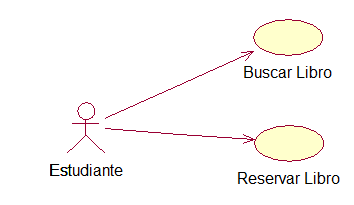
\includegraphics[width=10cm]{./Imagenes/img1} 
	\end{center}
	\item CASOS DE USO BIBLIOTECARIO .\\
		En el caso de uso del bilbiotecario se muestra la iteracion del bibliotecario con el sistema ya que el bibliotecario 	realiza los prestamos y tambien realiza el mantenimiento respectivo del sistema.
	\begin{center}
	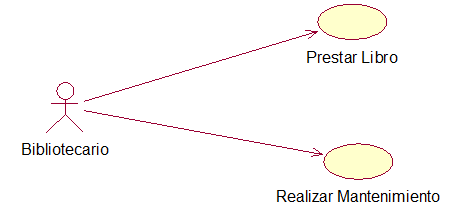
\includegraphics[width=10cm]{./Imagenes/img2} 
	\end{center}
\newpage
   	 \item DIAGRAMA DE SECUENCIA GENERAL DE PRESTAMO .\\
	\begin{center}
	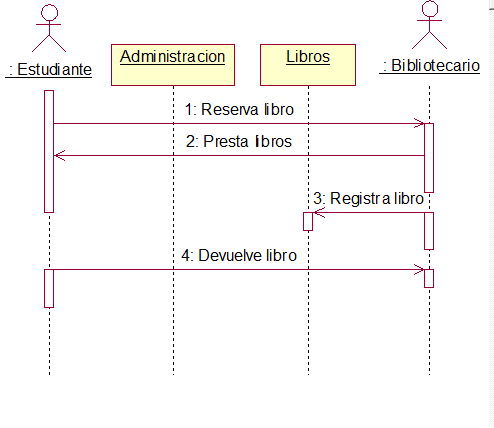
\includegraphics[width=12cm]{./Imagenes/img3} 
	\end{center}
	
\newpage
	\item DIAGRAMA DE SECUENCIA BIBLIOTECARIO .\\
	\begin{center}
	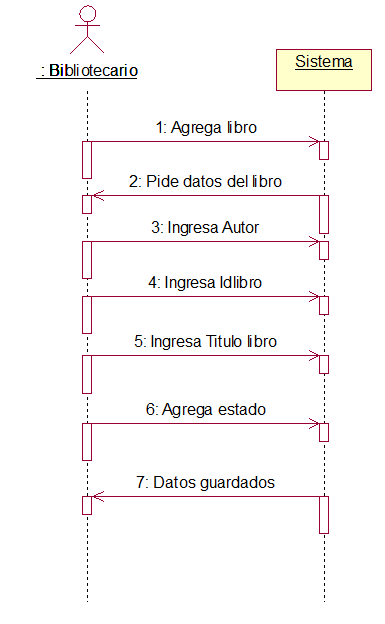
\includegraphics[width=12cm]{./Imagenes/img4} 
	\end{center}

\newpage
	\item DIAGRAMA DE SECUENCIA ESTUDIANTE .\\
	\begin{center}
	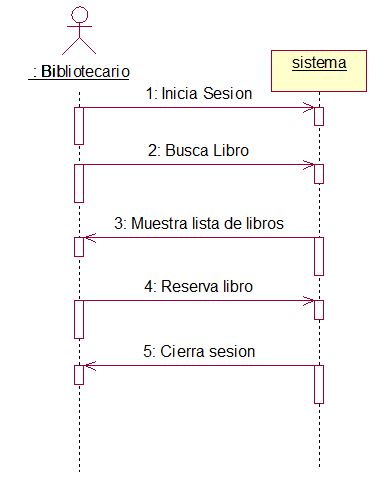
\includegraphics[width=12cm]{./Imagenes/img5} 
	\end{center}
	\newpage
\item DIAGRAMA DE ACTIVIDADES PRESTAMO DE LIBRO .\\
	\begin{center}
	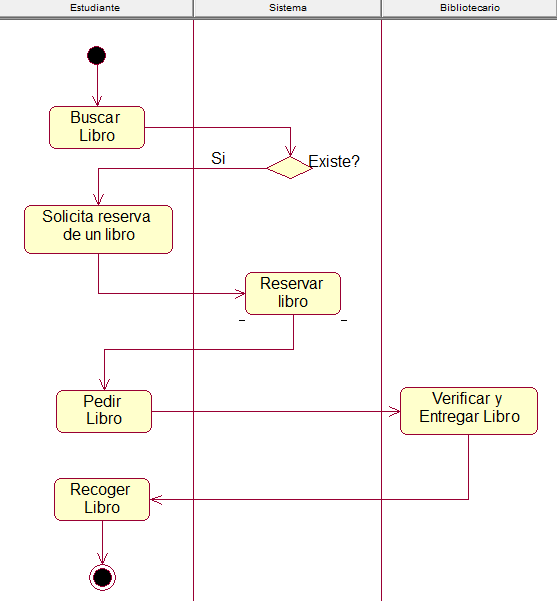
\includegraphics[width=12cm]{./Imagenes/img6} 
	\end{center}
\end{enumerate} 
